%%%%%%%%%%%%%%%%%%%%%%%%%%%%%%%%%%%%%%%%%%%%%%%%%%%%%%%%%%%%%%%%%%%%%%%%%%%%%%%%
\section{Android Overview}
%%%%%%%%%%%%%%%%%%%%%%%%%%%%%%%%%%%%%%%%%%%%%%%%%%%%%%%%%%%%%%%%%%%%%%%%%%%%%%%%
%------------------------------------------------------------------------------
\begin{frame}
\frametitle{Android Overview}
\alert{Android} is a comprehensive open source platform designed for mobile devices. It is championed by Google and owned by \href{http://www.openhandsetalliance.com/}{Open Handset Alliance}.
\begin{description}
	\item[Comprehensive] The Android SDK is all you need to start developing for Android.
	\item[Open Source Platform] Android is licensed under business-friendly licenses (Apache/MIT).
\end{description}
\end{frame}
%------------------------------------------------------------------------------
\subsection{History}
\begin{frame}
\frametitle{History}
\begin{enumerate}
	\item In 2005, Google buys Android Inc.
	\item In 2007, the Open Handset Alliance is announced.
	\item In 2008, the Android SDK 1.0 is released. The G1 phone, manufactured by HTC.
	\item 2009 sees a proliferation of Android-based devices. More than 20 devices run Android.
	\item In 2010, Android is second only to Blackberry as the best-selling smart phone platform. More than 60 devices that run Froyo.
\end{enumerate}
\end{frame}

%------------------------------------------------------------------------------
\subsection{Android Versions}
\begin{frame}
\frametitle{Android Versions}
\begin{table}[h]
\begin{tabular}{|c|c|c|c|} \hline
\multicolumn{4}{|c|}{\href{http://developer.android.com/about/dashboards/index.html}{Android Device Dashboard from 2013}} \\ \hline
Version & Codename &	API &	Distribution \\ \hline
1.6 & Donut & 4	& 0.2\% \\ \hline
2.1 & Eclair & 7 & 1.9\% \\ \hline
2.2 & Froyo  & 8 & 7.5\% \\ \hline
2.3 - 2.3.2 & \multirow{2}{*}{Gingerbread} & 9 &0.2\% \\
2.3.3 - 2.3.7 & & 10 & 43.9\% \\ \hline
3.1 & \multirow{2}{*}{Honeycomb} & 12 & 0.3\% \\
3.2 & & 13 & 0.9\% \\ \hline
4.0.3 - 4.0.4 & Ice Cream Sandwich & 15	& 28.6\% \\ \hline
4.1 & \multirow{2}{*}{Jelly Bean} & 16 & 14.9\% \\
4.2 & & 17 & 1.6\% \\ \hline
\end{tabular}
\caption{Data collected during a 14-day period ending on March 4, 2013.}
\end{table}
\end{frame}

%------------------------------------------------------------------------------
\subsection{The Stack}
\begin{frame}
\frametitle{The Stack}
\centering
\begin{columns}
\column{0.70\textwidth}
\centering
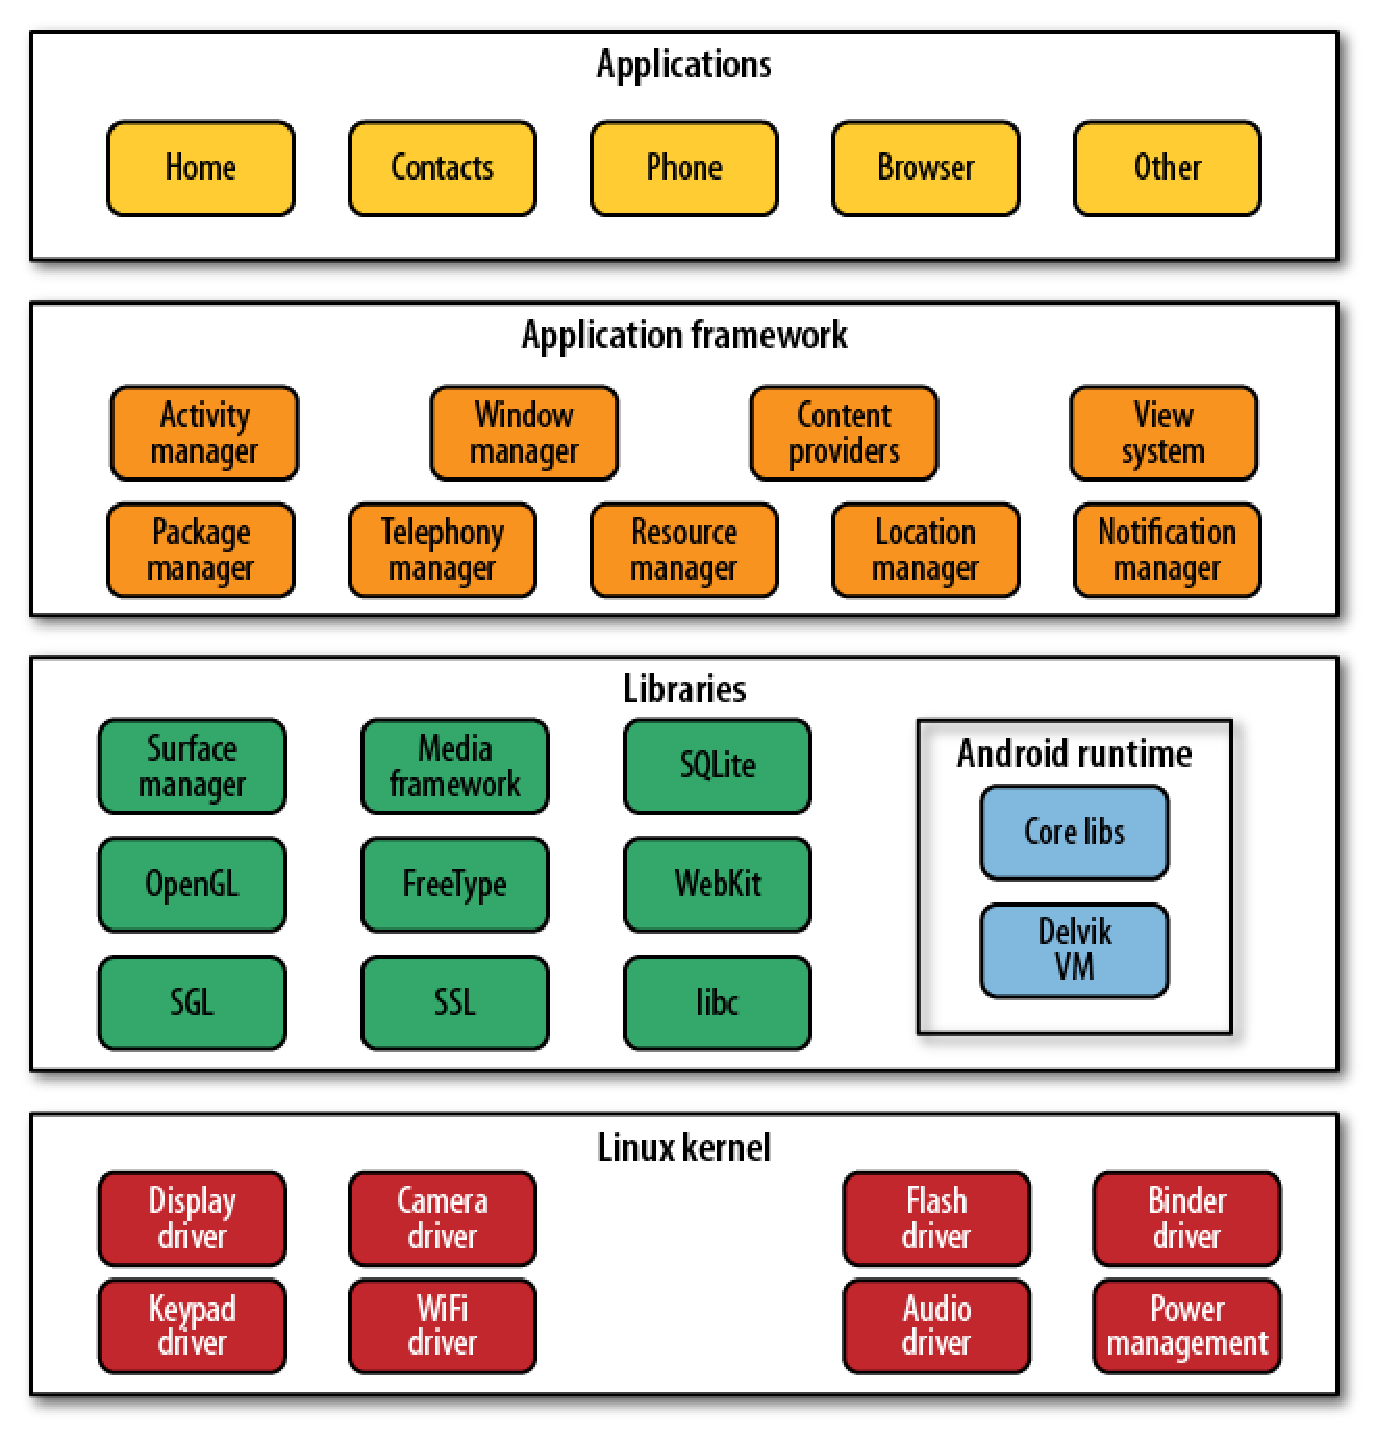
\includegraphics[width= 0.60 \textwidth]{fig-7.eps}
\column{0.45 \textwidth}
\begin{itemize}
\item Linux
\item Native Libraries
\item Dalvik
\item Application Framework
\item Applications
\end{itemize}


\end{columns}
\end{frame}

%------------------------------------------------------------------------------
\begin{frame}
\frametitle{Linux}
Android is built on top of \alert{Linux}.
\begin{description}
	\item[Portability] Linux is a portable platform that is relatively easy to compile on various hardware architectures
	\item[Security] All Android applications run as separate Linux processes with permissions set by the Linux system
	\item[Features] Memory management, power management, and networking
\end{description}
\end{frame}
%------------------------------------------------------------------------------
\begin{frame}
\frametitle{Native Libraries}
The \alert{native libraries} are C/C++ libraries, often taken from the open source community
in order to provide necessary services to the Android application layer. Among others,
they include:
\begin{description}
	\item[Webkit] A fast web-rendering engine used by Safari, Chrome, and other browsers
	\item[SQLite] A full-featured SQL database
	\item[Apache Harmony] An open source implementation of Java
	\item[OpenGL] 3D graphics libraries
	\item[OpenSSL] The secure locket layer
	\item[Bionic] A rewritten version of the standard C library
\end{description}
\end{frame}
%------------------------------------------------------------------------------
\begin{frame}
\frametitle{Dalvik, Android and  Java}
\alert{Dalvik} is a purpose-built virtual machine designed specifically for Android, developed
by Dan Bornstein and his team at Google
\centering
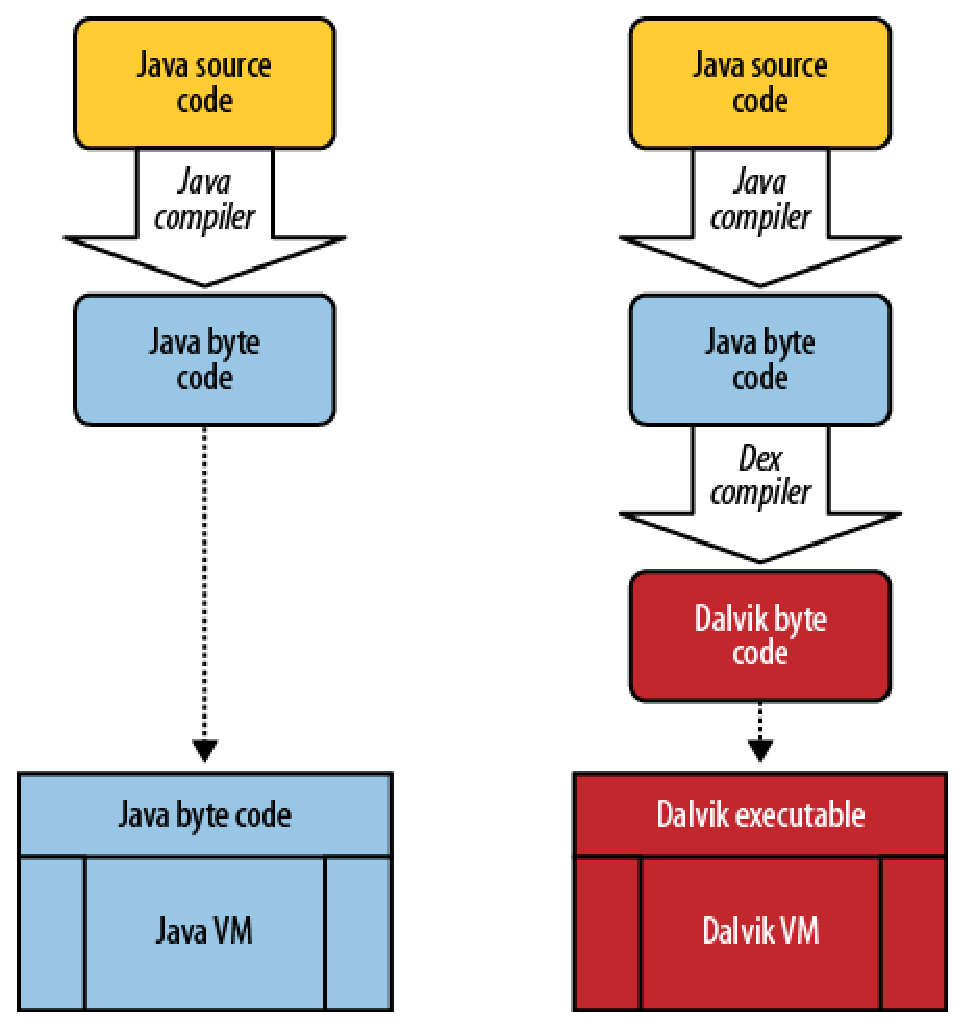
\includegraphics[width= 0.40 \linewidth]{fig-9.eps}
\end{frame}
%------------------------------------------------------------------------------
\begin{frame}
\frametitle{Application Framework}
The \alert{application framework} is a rich environment that provides numerous services to
help you, the app developer, get your job done
\begin{columns}
\column{0.65 \textwidth}
\centering
\includegraphics[width= 1.0 \textwidth]{fig-2001.eps}
\end{columns}
\end{frame}
%------------------------------------------------------------------------------
\begin{frame}
\frametitle{Applications}
An \alert{application} is a single application package (APK) file. An APK file roughly has three
main components:
\begin{description}
	\item[Dalvik executable] Java source code compiled down to a Dalvik executable
	\item[Resources] Resources are everything that is not code (images, audio/video clips, XML files describing layouts, language packs \dots
	\item[Native libraries] Your application may include some native code, such as C/C++ libraries
\end{description}
\end{frame}
%------------------------------------------------------------------------------
\subsection[Plattform Set Up]{Plattform Set Up}
\begin{frame}
\frametitle{Plattform Set Up}
\begin{enumerate}
 	\item Install the Android SDK, \href{http://developer.android.com/sdk/index.html}{Android SDK Download page}
	\item Install the Platform-tools, using the SDK Manager \texttt{tools/android update sdk --no-ui}
	\item Install Eclipse, \href{http://www.eclipse.org/downloads}{Eclipse IDE for Java Developers}
	\item Instal Android Tool for Eclipse (Android DDMS and Android Development Tools), \url{https://dl-ssl.google.com/android/}

\end{enumerate}
\end{frame}
%------------------------------------------------------------------------------
\subsection{Hello World!}

%------------------------------------------------------------------------------
\begin{frame}
\frametitle{Hello Wolrd!}
\begin{columns}
\column{0.5 \textwidth}
\centering
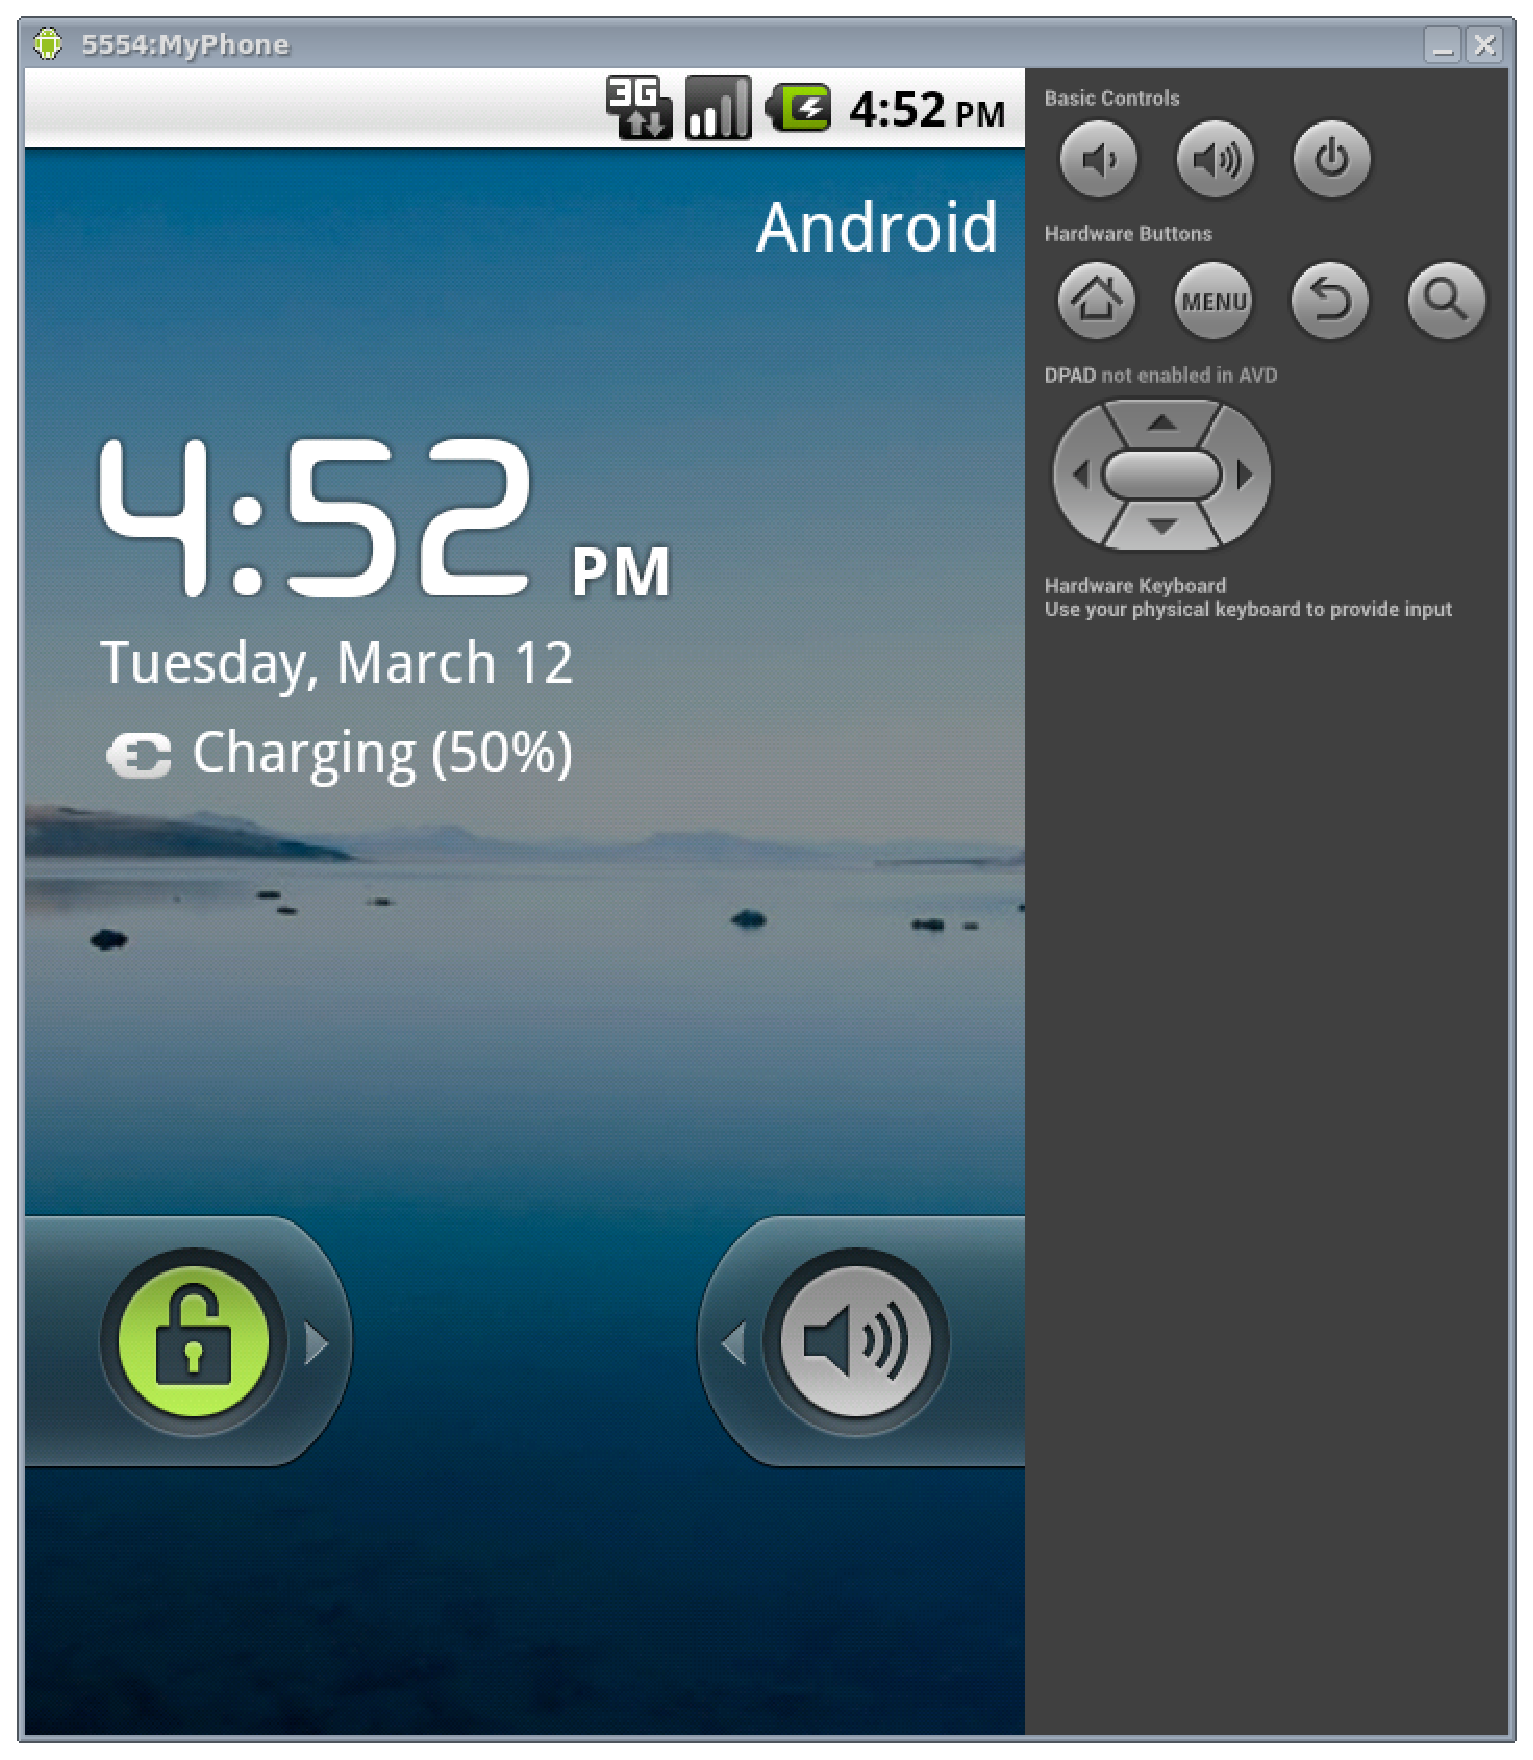
\includegraphics[width= 1.0 \textwidth]{MyPhone.eps}
\column{0.5 \textwidth}
\centering
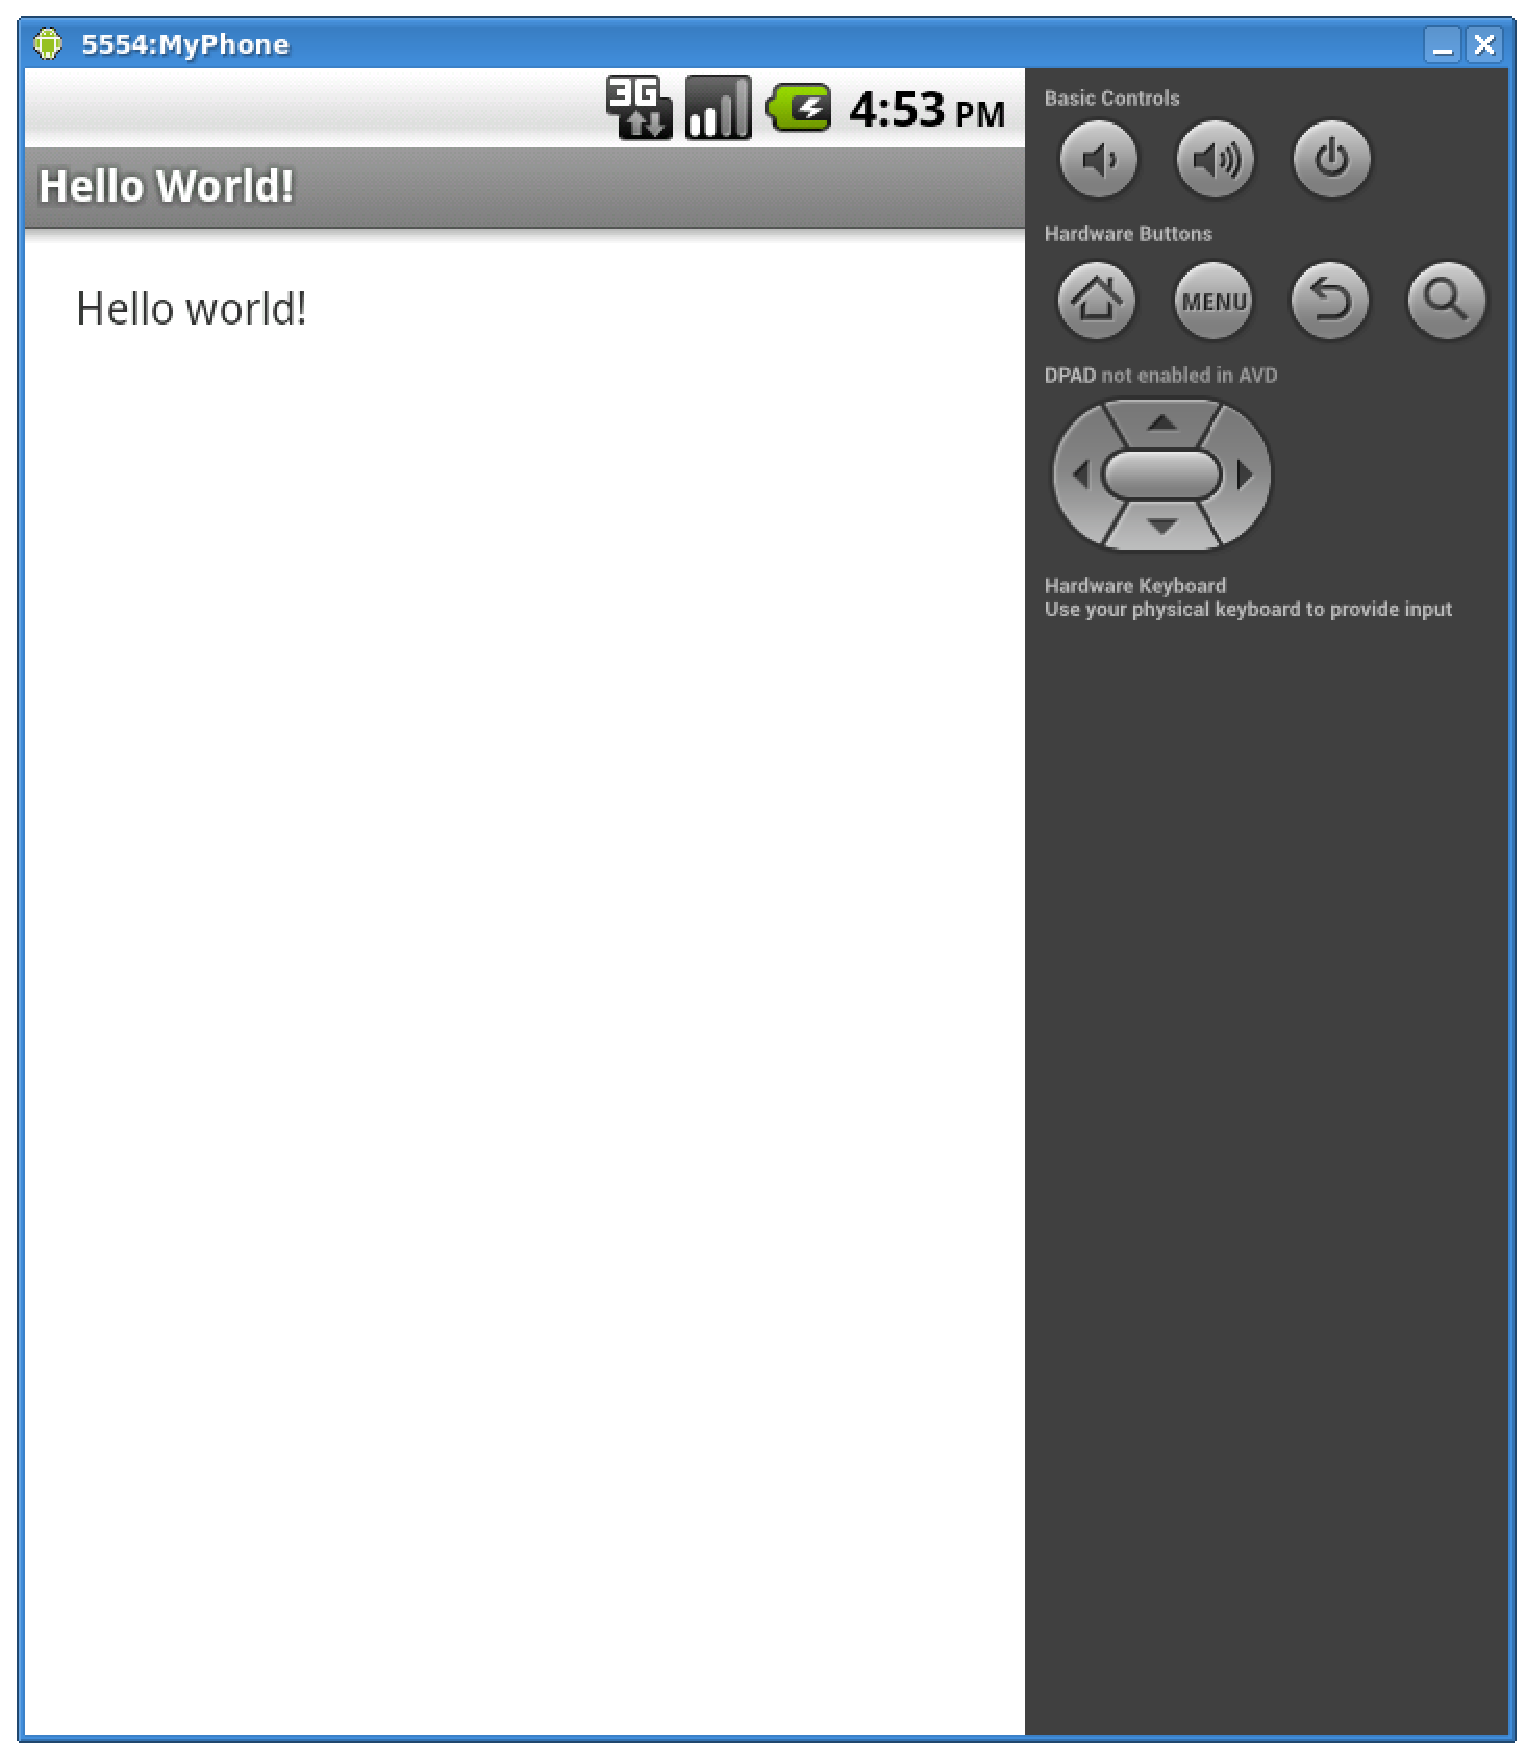
\includegraphics[width= 1.0 \textwidth]{HelloWorld.eps}
\end{columns}
\end{frame}
%------------------------------------------------------------------------------

\begin{frame}
\frametitle{Creating a New Project}
\textbf{File|New Android Application Project}\\
\alert{Application Name}, \alert{Project Name}, \alert{Package Name}

\begin{columns}
\column{0.45 \textwidth}
\centering
\includegraphics[width= 1.0 \textwidth]{NewAndroidApplication1.eps}
\column{0.65 \textwidth}
\begin{description}
 	\item[Application Name] \textbf{Hello World!} The application name is the plain English name of your application
	\item[Project Name] \textbf{HelloWorld} Eclipse organizes everything into projects. A project name should be one word
	\item[Package Name] \textbf{com.artemisa} In Java, all source code is organized into packages
\end{description}
\end{columns}
\end{frame}
%------------------------------------------------------------------------------
\begin{frame}[fragile]
\frametitle{Manifiest File}
The manifest file explains what the application consists of
\lstset{language=XML, style=eclipse}
\begin{adjustbox}{width=0.8 \textwidth}
\begin{lstlisting}[caption=AndroidManifiest.xml]
<?xml version="1.0" encoding="utf-8"?>
<manifest xmlns:android="http://schemas.android.com/apk/res/android"
    package="com.artemisa.helloworld"
    android:versionCode="1"
    android:versionName="1.0" >

    <uses-sdk
        android:minSdkVersion="8"
        android:targetSdkVersion="17" />

    <application
        android:allowBackup="true"
        android:icon="@drawable/ic_launcher"
        android:label="@string/app_name"
        android:theme="@style/AppTheme" >
        <activity
            android:name="com.artemisa.helloworld.MainActivity"
            android:label="@string/app_name" >
            <intent-filter>
                <action android:name="android.intent.action.MAIN" />

                <category android:name="android.intent.category.LAUNCHER" />
            </intent-filter>
        </activity>
    </application>

</manifest>
\end{lstlisting}
\end{adjustbox}
\end{frame}
%------------------------------------------------------------------------------
\begin{frame}[fragile]
\frametitle{Layout XML Code}
The layout file specifies the layout of your screen. Layout XML is responsible for the layout of widgets
\lstset{language=XML, style=eclipse}
\begin{adjustbox}{width=1.0 \textwidth}
\begin{lstlisting}[caption=res/layout/activity\_main.xml]
<RelativeLayout xmlns:android="http://schemas.android.com/apk/res/android"
    xmlns:tools="http://schemas.android.com/tools"
    android:layout_width="match_parent"
    android:layout_height="match_parent"
    android:paddingBottom="@dimen/activity_vertical_margin"
    android:paddingLeft="@dimen/activity_horizontal_margin"
    android:paddingRight="@dimen/activity_horizontal_margin"
    android:paddingTop="@dimen/activity_vertical_margin"
    tools:context=".MainActivity" >

    <TextView
        android:layout_width="wrap_content"
        android:layout_height="wrap_content"
        android:text="@string/hello_world" />

</RelativeLayout>
\end{lstlisting}
\end{adjustbox}
\end{frame}
%------------------------------------------------------------------------------
\begin{frame}[fragile]
\frametitle{Strings}
This is another XML file that contains all the text that your application uses. Strings XML is responsible for their textual content
\lstset{language=XML, style=eclipse}
\begin{adjustbox}{width=1.0 \textwidth}
\begin{lstlisting}[caption=res/values/strings.xml]
<?xml version="1.0" encoding="utf-8"?>
<resources>

    <string name="app_name">Hello World!</string>
    <string name="action_settings">Settings</string>
    <string name="hello_world">Hello world!</string>

</resources>
\end{lstlisting}
\end{adjustbox}
\end{frame}
%------------------------------------------------------------------------------
\begin{frame}[fragile]
\frametitle{The R file}
The R file is the glue between Java and the resources
\lstset{language=java, style=eclipse, tabsize=2}
\begin{adjustbox}{width=0.5 \textwidth}
\begin{lstlisting}[caption=gen/artemisa/helloworld/R.java]
/* AUTO-GENERATED FILE.  DO NOT MODIFY.
 *
 * This class was automatically generated by the
 * aapt tool from the resource data it found.  It
 * should not be modified by hand.
 */

package com.artemisa.helloworld;

public final class R {
    public static final class attr {
    }
    public static final class dimen {
        /**  Default screen margins, per the Android Design guidelines. 

         Customize dimensions originally defined in res/values/dimens.xml (such as
         screen margins) for sw720dp devices (e.g. 10" tablets) in landscape here.
    
         */
        public static final int activity_horizontal_margin=0x7f040000;
        public static final int activity_vertical_margin=0x7f040001;
    }
    public static final class drawable {
        public static final int ic_launcher=0x7f020000;
    }
    public static final class id {
        public static final int action_settings=0x7f080000;
    }
    public static final class layout {
        public static final int activity_main=0x7f030000;
    }
    public static final class menu {
        public static final int main=0x7f070000;
    }
    public static final class string {
        public static final int action_settings=0x7f050001;
        public static final int app_name=0x7f050000;
        public static final int hello_world=0x7f050002;
    }
    // ...
}
\end{lstlisting}
\end{adjustbox}
\end{frame}
%------------------------------------------------------------------------------
\begin{frame}[fragile]
\frametitle{Java Source Code}
The Java code is what drives everything. This is the code that ultimately gets converted
to a Dalvik executable and runs your application
\lstset{language=java, style=eclipse, tabsize=2}
\begin{adjustbox}{width=0.85 \textwidth}
\begin{lstlisting}[caption=src/com/artemisa/helloworld/MainActivity.java]
package com.artemisa.helloworld;

import android.os.Bundle;
import android.app.Activity;
import android.view.Menu;

public class MainActivity extends Activity {

	@Override
	protected void onCreate(Bundle savedInstanceState) {
		super.onCreate(savedInstanceState);
		setContentView(R.layout.activity_main);
	}

	@Override
	public boolean onCreateOptionsMenu(Menu menu) {
		// Inflate the menu; this adds items to the action bar if it is present.
		getMenuInflater().inflate(R.menu.main, menu);
		return true;
	}

}
\end{lstlisting}
\end{adjustbox}
\end{frame}
%------------------------------------------------------------------------------
\begin{frame}
\frametitle{The Emulator}
To use the emulator, we’ll have to create an Android Virtual Device (AVD)
\begin{columns}
\column{1.0 \textwidth}
\centering
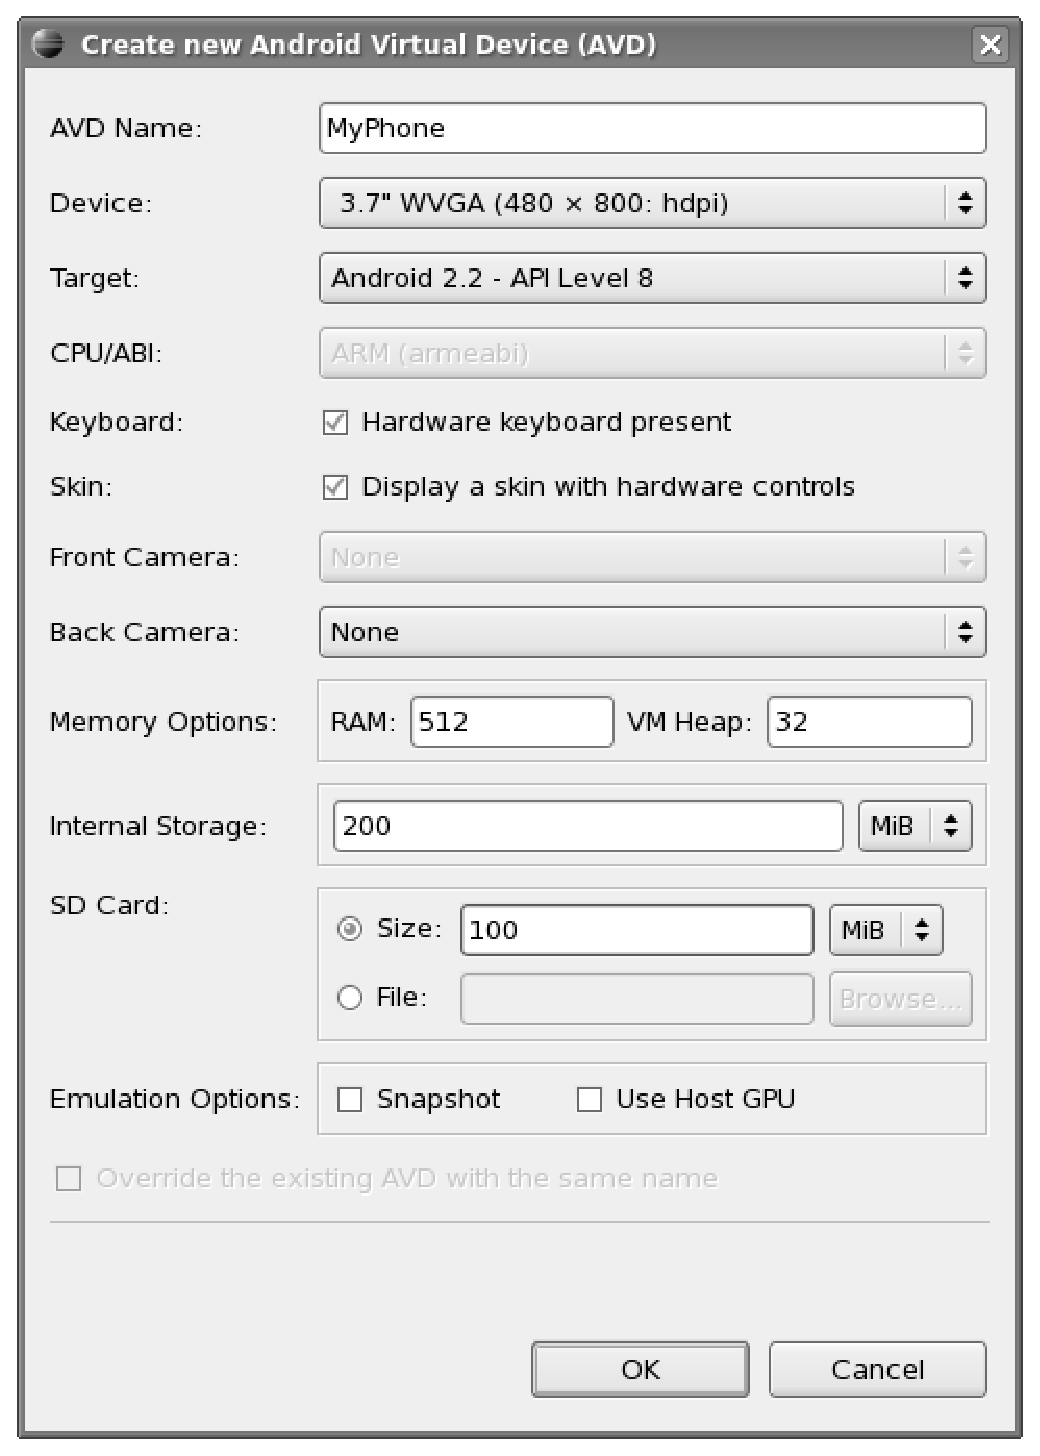
\includegraphics[width= 0.35 \textwidth]{CreateNewAndroidVitualDevice.eps}
\end{columns}
\end{frame}
%------------------------------------------------------------------------------
\begin{frame}
\frametitle{Go Ahead and Be Patient!}
\begin{columns}
\column{0.5 \textwidth}
\centering
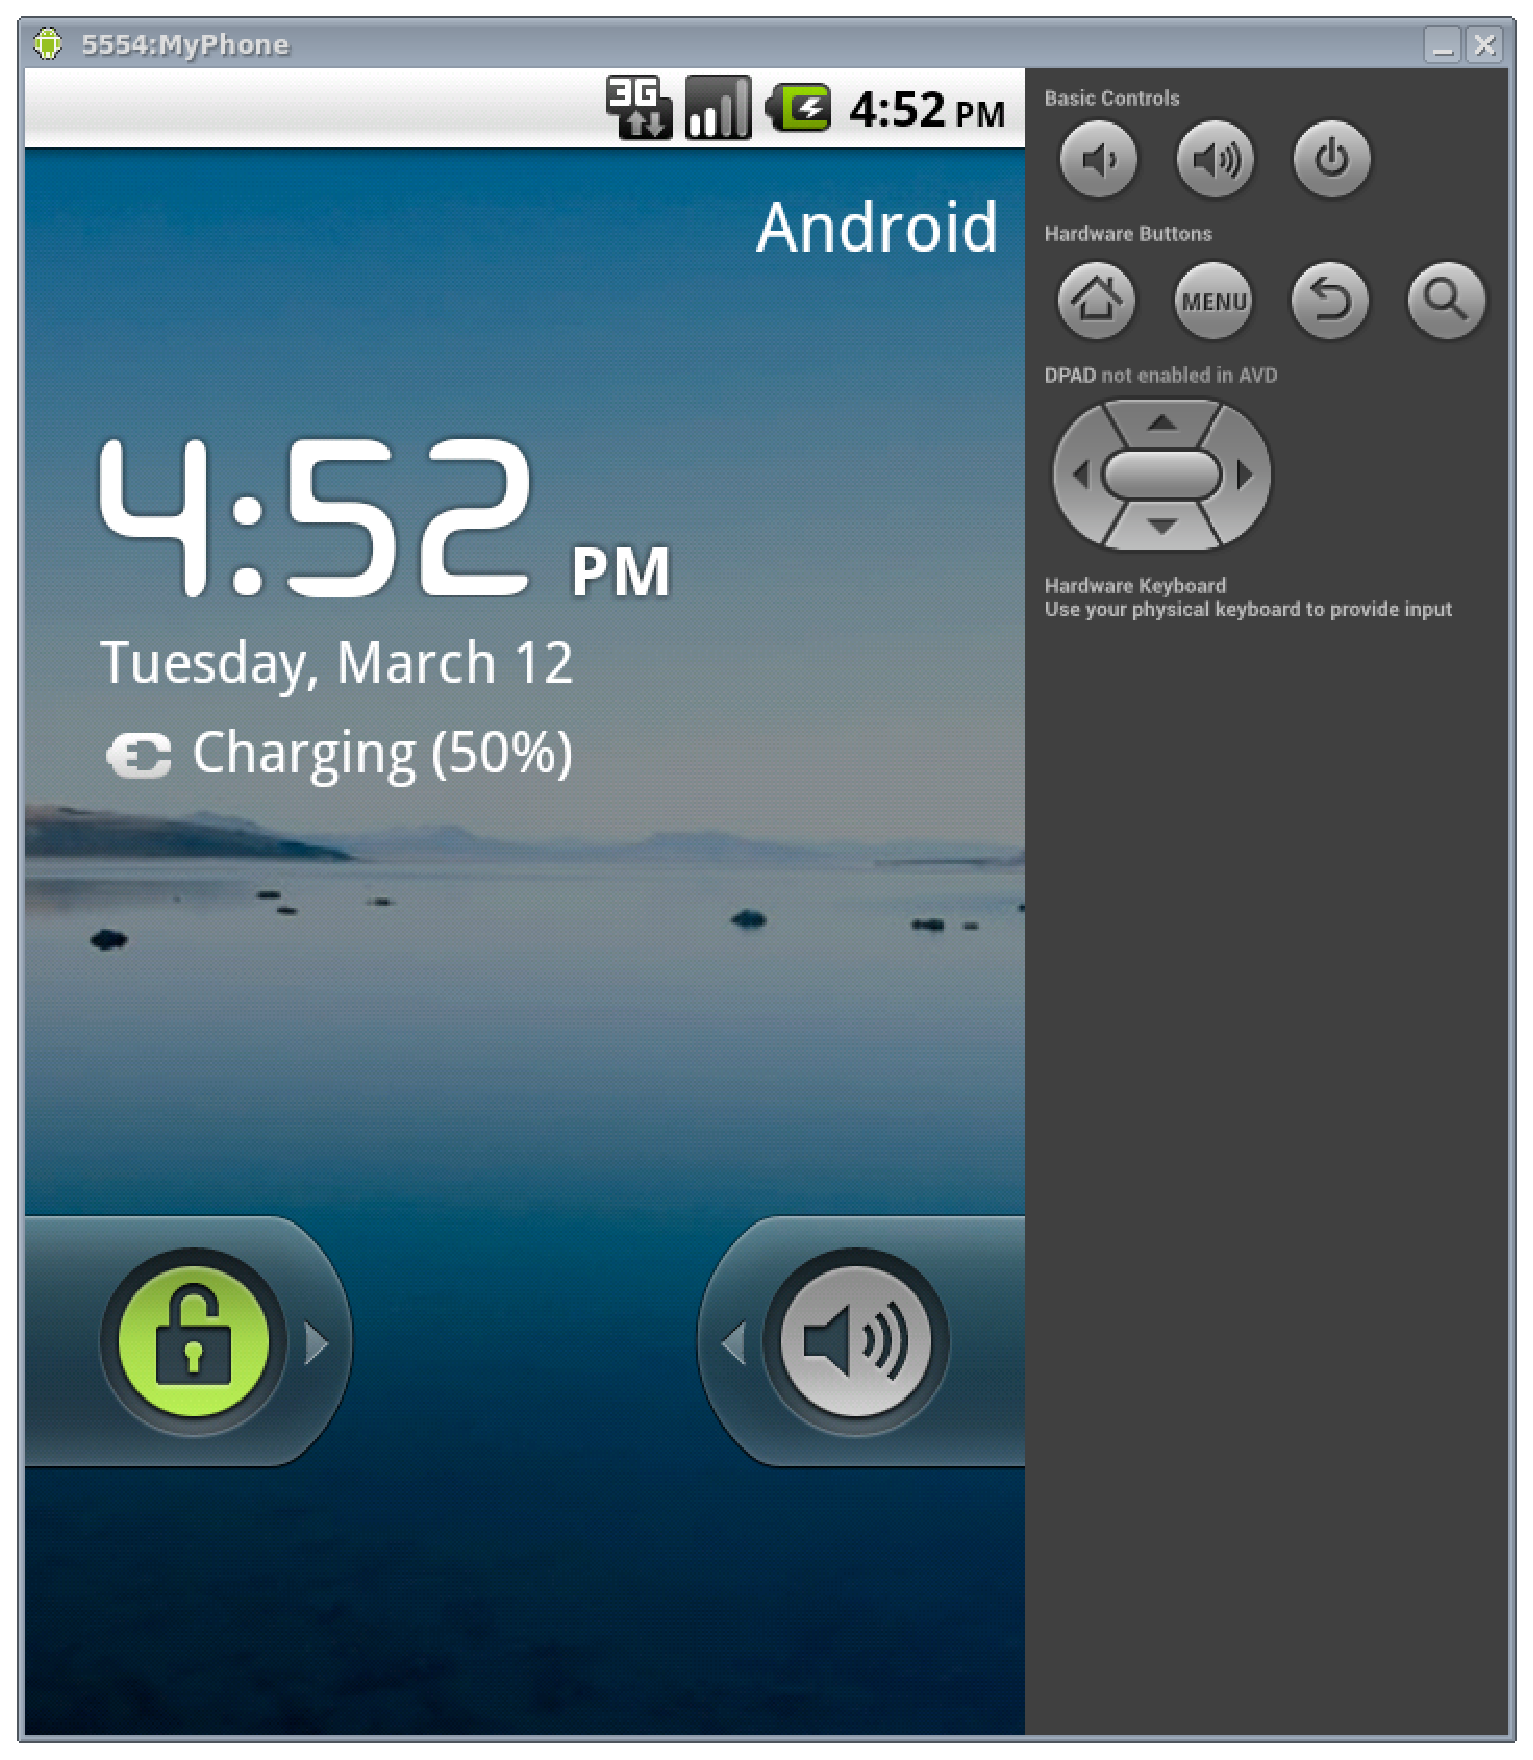
\includegraphics[width= 1.0 \textwidth]{MyPhone.eps}
\column{0.5 \textwidth}
\centering
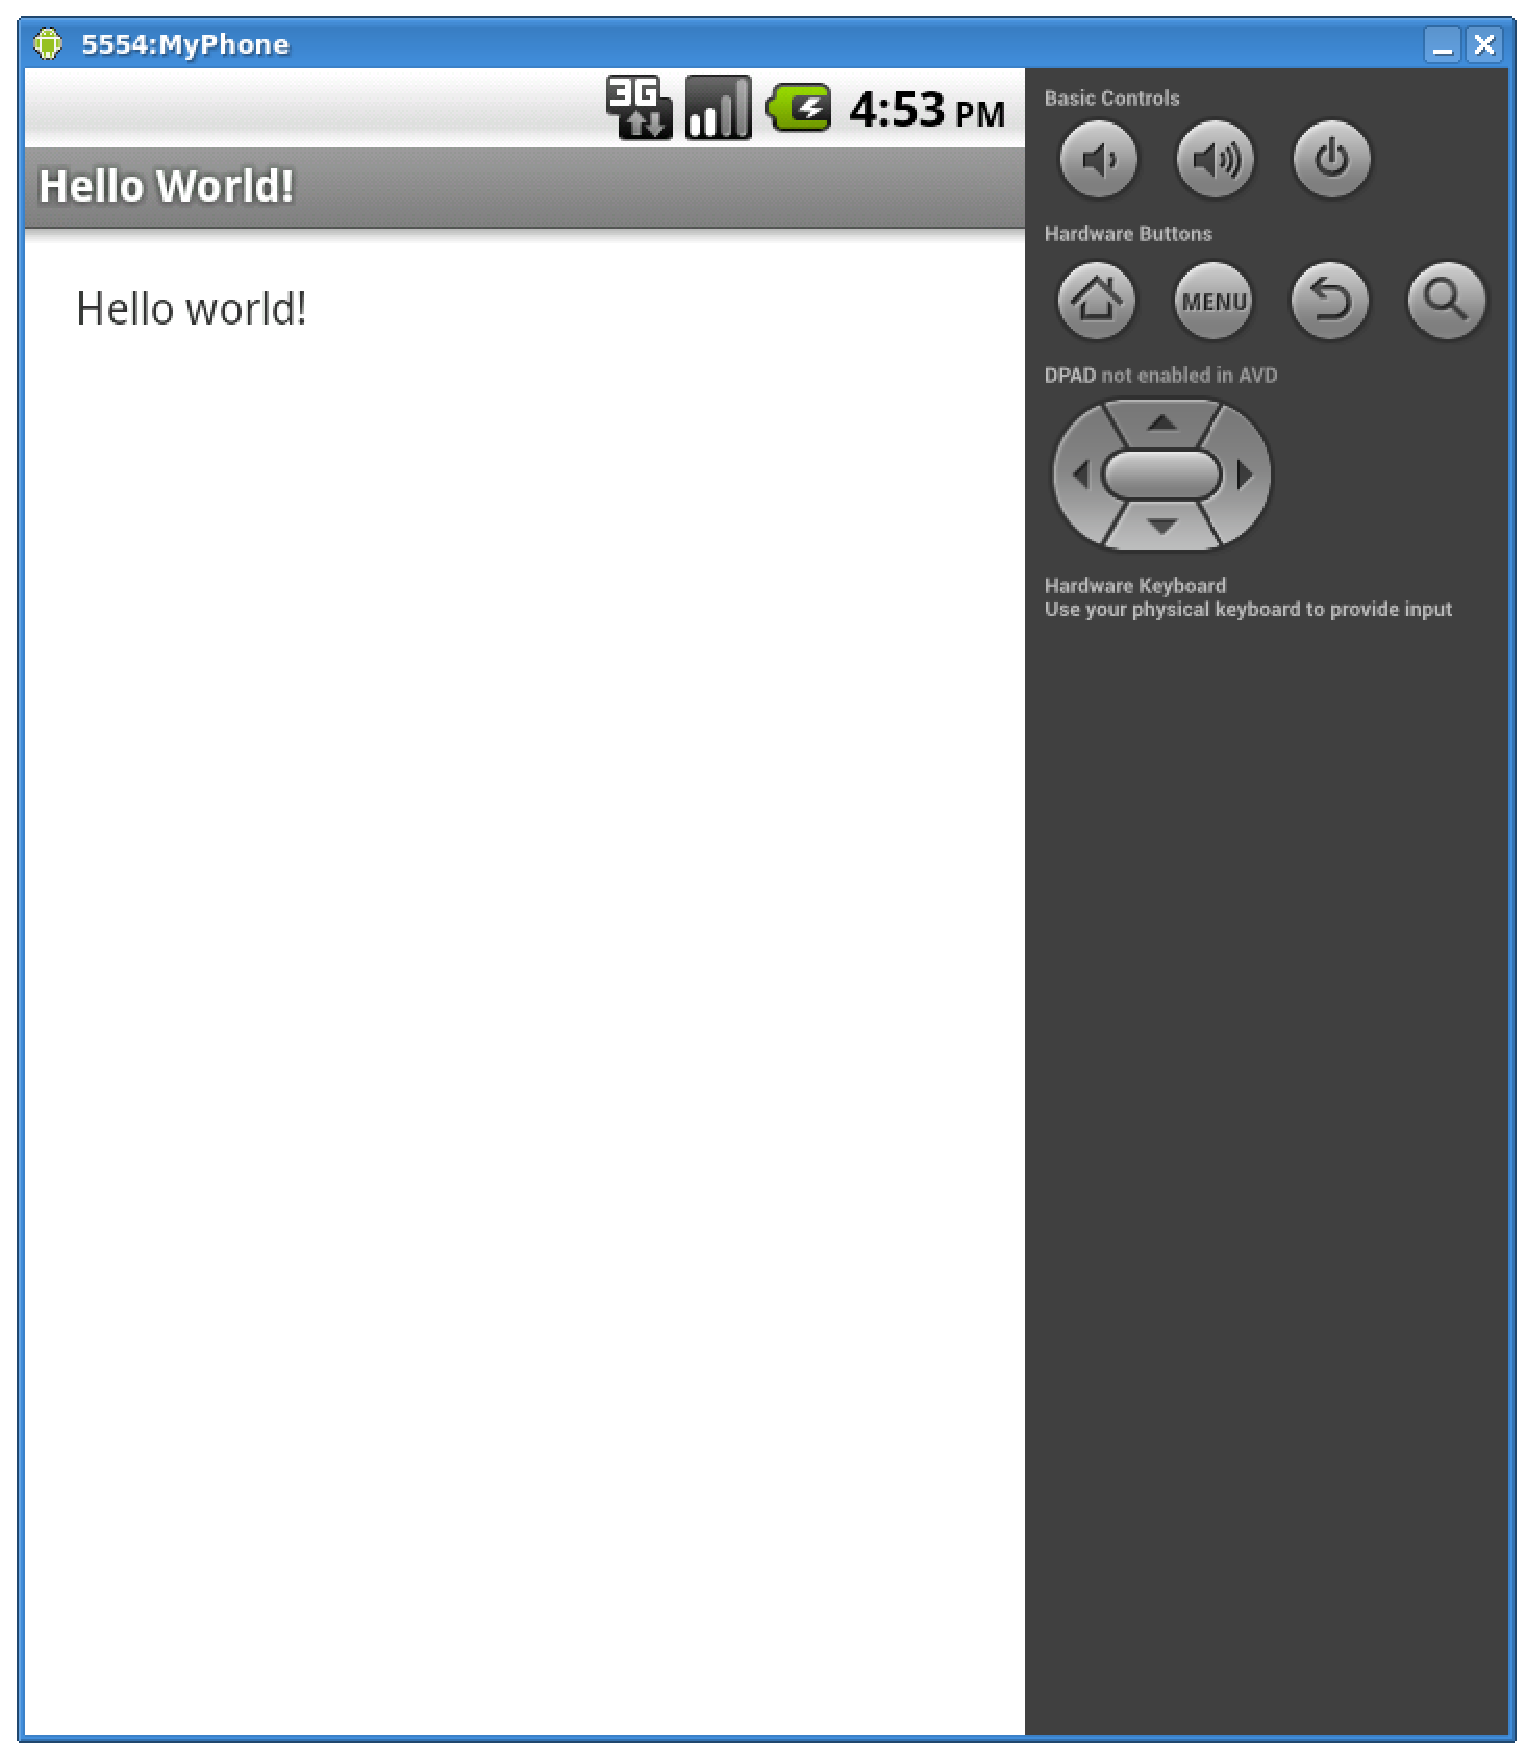
\includegraphics[width= 1.0 \textwidth]{HelloWorld.eps}
\end{columns}
\end{frame}
%------------------------------------------------------------------------------
\subsection{The Yamba Application}
%------------------------------------------------------------------------------
\begin{frame}
\frametitle{Yet Another Micro Blogging App}
\begin{columns}
 \column{0.33 \textwidth}
	\begin{figure}
	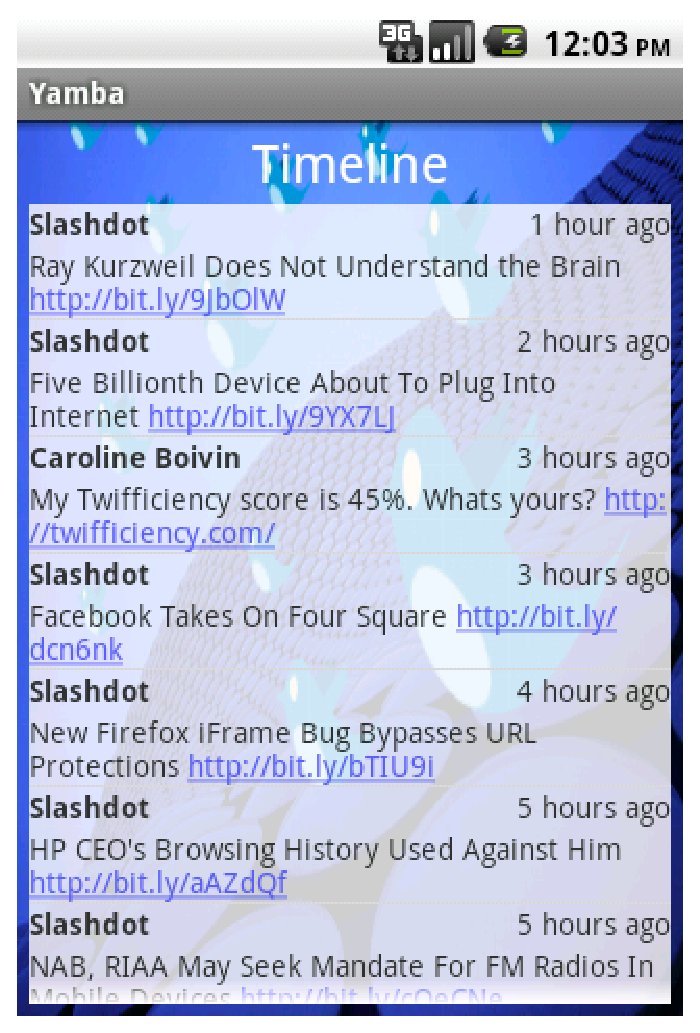
\includegraphics[width= 0.8 \textwidth]{fig-30.eps}
	\caption{List of status messages from other people, called a timeline}
	\end{figure}
 \column{0.33 \textwidth}
	\begin{figure}
	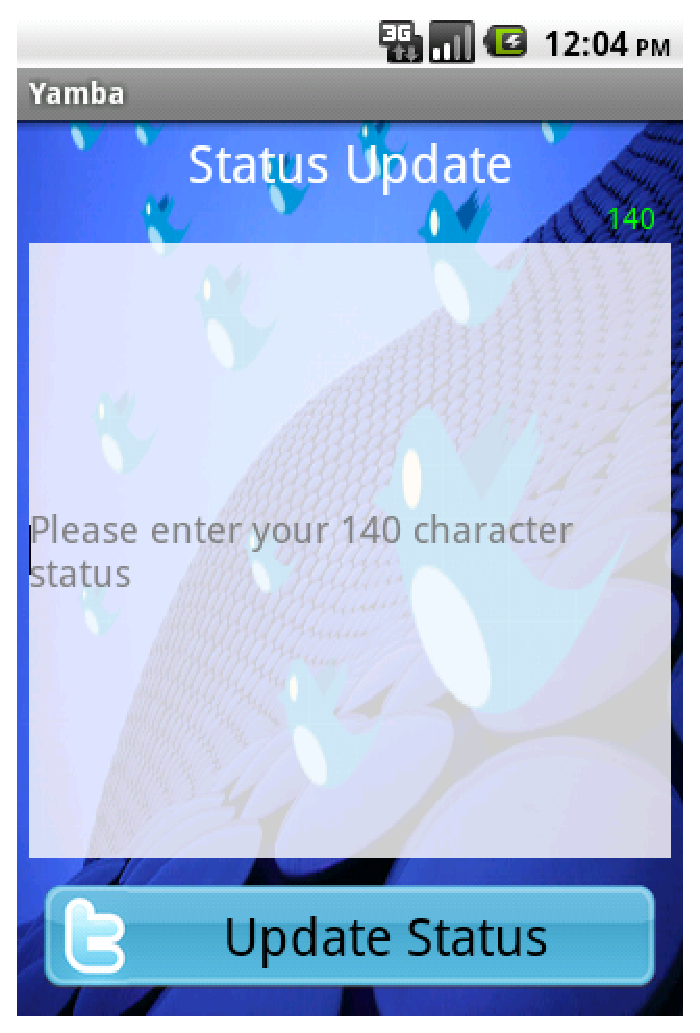
\includegraphics[width= 0.8 \textwidth]{fig-31.eps}
	\caption{Screen where the user can enter a status message}
	\end{figure}
 \column{0.34 \textwidth}
	\begin{figure}
	\includegraphics[width= 0.8 \textwidth]{fig-32.eps}
	\caption{User preferences}
	\end{figure}
\end{columns}

\end{frame}
%------------------------------------------------------------------------------
